
\chapter{Conclusions and Future Work}
\label{Chapter6}

\section{Conclusions}

\subsection{Low force output}
In the previous chapter, we measured the \textbf{maximum force} our system could generate in the \textbf{best conditions}.
Even \textbf{overloading} the coil for short bursts of \textbf{30V} we achieved a measle \textbf{$5\cdot10^{-5}$N} of force \ref{subsubsec: Magnet_size_vs_Force}.
Considering the \textbf{small magnet prototype} (\textbf{1.03g} mass), this means we have generated an \textbf{acceleration} of about \textbf{0.05m/s\textsuperscript{2}}.
The \textbf{application area} is about \textbf{78.54mm\textsuperscript{2}}, so considering what we discussed in paragraph \ref{Haptic sensitivity}, the prototype couldn't even reach the haptic sensitivity of human fingers (\textbf{[0.1778-0.5623]m/s\textsuperscript{2}}).

Test subjects were \textbf{anyway able to feel some vibrations}, we can theorize that the sensitivity threshold was \textbf{lowered} by the \textbf{constant pressure force} applied on the skin by the \textbf{membrane} (\textbf{0.2N}), this is also supported by the study in paragraph \ref{Haptic sensitivity}.
The vibrations were still \textbf{very weak} and \textbf{barely perceptible}.

\subsection{Alternative signals}
We also tested other \textbf{low RMS signals} with \textbf{high peaks} to see if we could simulate \textbf{other sensations} besides the heartbeat.
We tested the sound of \textbf{gunshots}, the sound of a \textbf{bell ringing} and the sound of a \textbf{thunder strike}.
The best result was achieved with the thunder strike, the \textbf{big peak} created a \textbf{satisfying vibration} and we could even tell somewhat the consequent \textbf{rumbles}.
The only problem was that subjects\textbf{ weren't able to recognize what the vibration was supposed to represent} without being told beforehand, that wasn't the case with the heartbeat.

\subsection{A technology not suitable for haptic feedback devices}
As we discussed multiple times in this thesis, driving these low-resistance flexible coils with \textbf{AC signals} is very \textbf{difficult} and \textbf{inefficient}.
The complex circuitry required to drive these coils is not only \textbf{expensive} but also \textbf{difficult to design and tune}.
The high power consumption is also a major drawback.
Combining all these factors with the low magnetic field output, we can conclude that this technology is \textbf{not ready for mainstream application in haptic feedback devices}.

\section{Alternative applications}
The most promising application for flexible PCB coils is using them as very \textbf{thin electromagnets}.
By combining them with \textbf{high magnetic permeability materials}, we could increase substantially their \textbf{magnetic field output} \ref{Magnetic field generation}.
Usually, high-permeability materials are metals so we could also exploit their \textbf{high thermal conductivity} to \textbf{dissipate the heat} generated by the coils, allowing us to increase the coil power input and in turn their magnetic field output.
Some tests in this direction have already been done in the past \cite{Flexar_as_electromagnets}.

Meanwhile, a very interesting application for standard PCB coils is PCB stator axial electric motors.
This type of motor has multiple advantages over traditional electric ones:
\begin{itemize}
    \item \textbf{Very thin} and \textbf{lightweight} stators.
    \item \textbf{Very low inertia}, allowing for very \textbf{fast response times}.
    \item \textbf{High efficiency}.
    \item \textbf{Lower cost} and \textbf{material waste} as we have no need for copper windings.
    \item \textbf{High reliability} as windings are usually prone to \textbf{mechanical failure}.
    \item \textbf{Ease of repair} as we can easily replace the PCB.
    \item \textbf{Easy customization} as by changing the stator PCB design, one can modify the \textbf{torque-speed curve} of the motor and \textbf{size} of the motor. Also by increasing the \textbf{number of layers of the PCB}, we can increase the stator \textbf{magnetic field output}.
\end{itemize}

\begin{figure}[H]
    \centering
    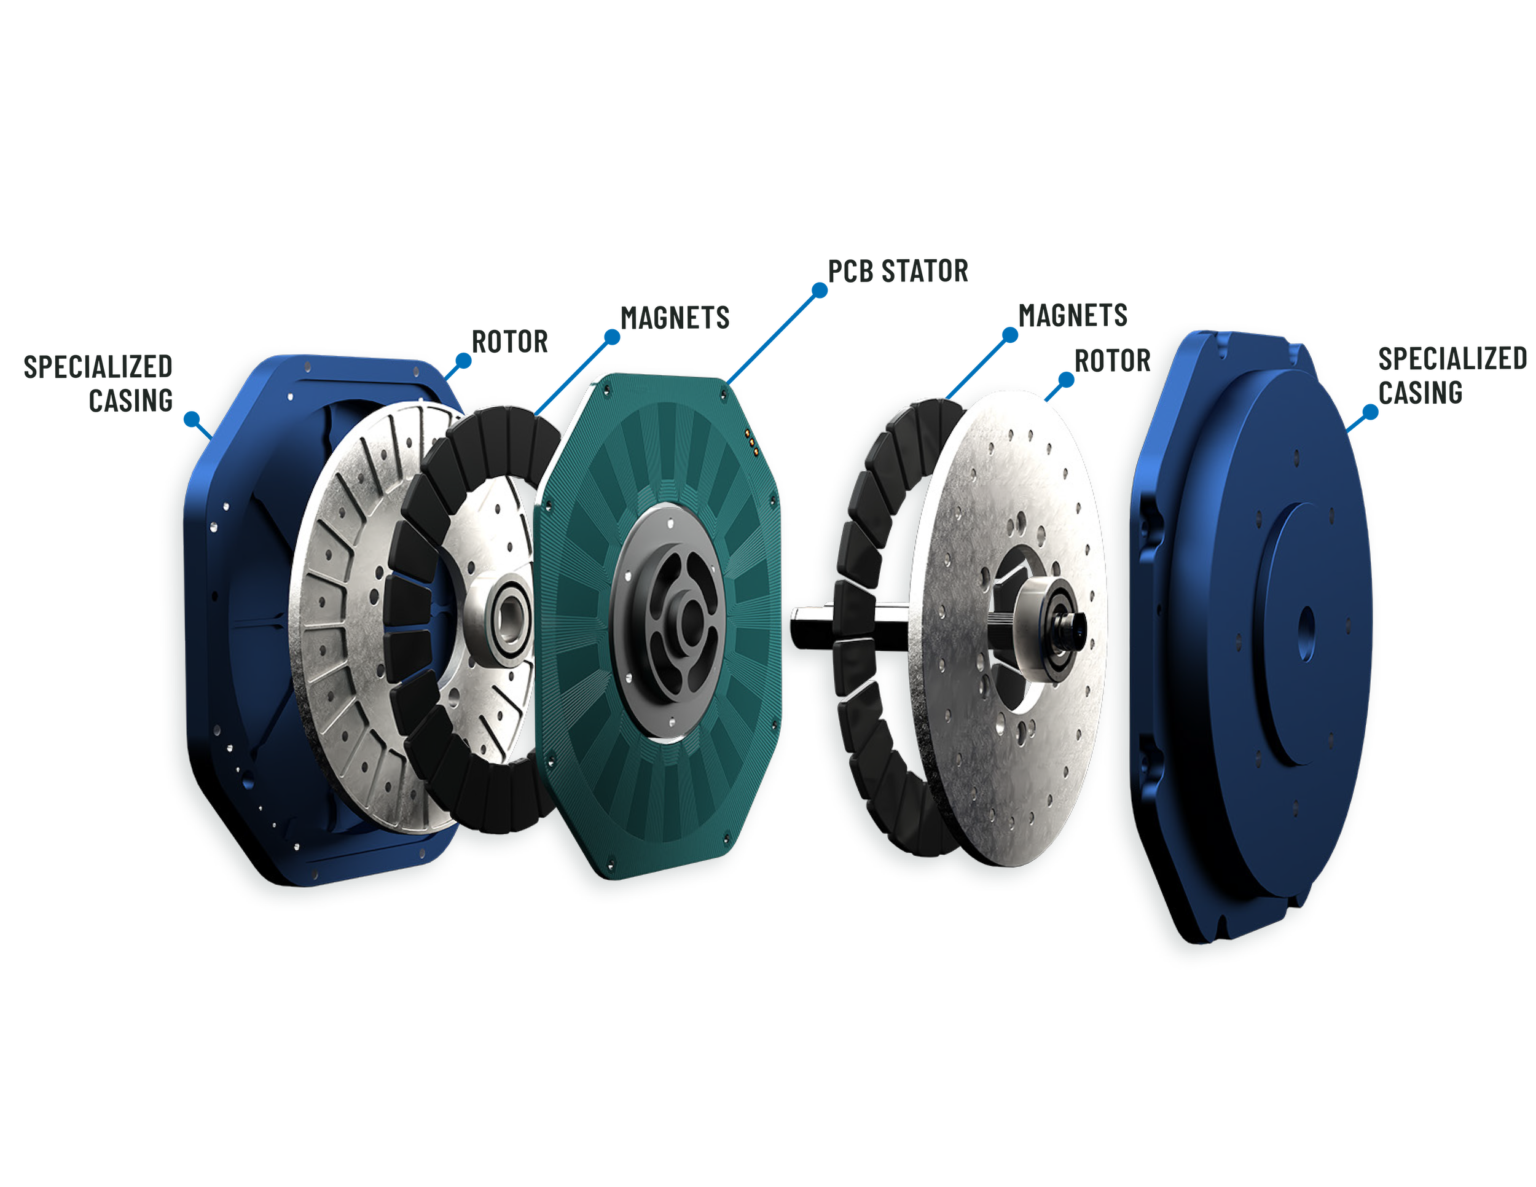
\includegraphics[width=0.8\textwidth]{Chapters/Chapter6/Figures/PCB_stator_motor_expl.png}
    \caption{Explosion view of a PCB stator axial motor from PCB Stator \cite{PCBStator}.}
    \label{fig:PCB_motor}
\end{figure}

\section{Future work}
Some effort could be put into \textbf{optimizing the coil design} for haptic feedback applications.
We could especially focus on \textbf{increasing the magnetic field output} of the coils and optimizing the \textbf{magnetic field coupling} with the magnet.

\subsection{Custom coil design}
As we previously briefly touched on, PBC coils can be designed with \textbf{very different traces design} in mind \ref{subsec: Planar_coils}.
One way to exploit this could be to \textbf{increase the number of spires in the same area}, increasing the magnetic field output.
For example, considering Flexar coils, we could use a \textbf{square pattern} for the traces to increase the number of spires in the same area.
Then we could substitute the cylindrical magnet with a \textbf{parallelepiped one}, to increase the m\textbf{agnetic field coupling with the coil}.

This is all speculation in fact, it could be wise to first due some \textbf{FEM simulations} to test the feasibility of this idea.